%%%%%%%%%%%%%%%%%%%%%%%%%%%%%%%%%%%%%%%%%%%%%%%%%%%%%%%%%%%%%%%%%%%%%
% LaTeX Template: Project Titlepage Modified (v 0.1) by rcx
%
% Original Source: http://www.howtotex.com
% Date: February 2014
% 
% This is a title page template which be used for articles & reports.
% 
% This is the modified version of the original Latex template from
% aforementioned website.
% 
%%%%%%%%%%%%%%%%%%%%%%%%%%%%%%%%%%%%%%%%%%%%%%%%%%%%%%%%%%%%%%%%%%%%%%

\documentclass[12pt]{report}
\usepackage[a4paper]{geometry}
\usepackage[myheadings]{fullpage}
\usepackage{fancyhdr}
\usepackage{lastpage}
\usepackage{graphicx, wrapfig,setspace, booktabs}
\usepackage[T1]{fontenc}
\usepackage[font=small, labelfont=bf]{caption}
\usepackage{fourier}
\usepackage[protrusion=true, expansion=true]{microtype}
\usepackage[english]{babel}
\usepackage{sectsty}
\usepackage{lipsum}
\usepackage[hyphens]{url}
%\usepackage{subfig}
\usepackage{hyperref}
\usepackage{alphalph}
\usepackage[utf8]{inputenc}
\usepackage{multicol}
\usepackage{amsmath}
\usepackage{subfigure}
\renewcommand*{\thesubfigure}{%
\alphalph{\value{subfigure}}%
}%


\newcommand{\HRule}[1]{\rule{\linewidth}{#1}}
\onehalfspacing
\setcounter{tocdepth}{5}
\setcounter{secnumdepth}{5}
\usepackage{float}

\usepackage[backend=bibtex,style=chem-acs,biblabel=dot]{biblatex}
\addbibresource{references.bib}

%-------------------------------------------------------------------------------
% HEADER & FOOTER
%-------------------------------------------------------------------------------
\pagestyle{fancy}
\fancyhf{}
\setlength\headheight{15pt}
\fancyhead[L]{CS7015: PA3}
\fancyhead[R]{Deep Learning}
\fancyfoot[R]{Page \thepage\ of \pageref{LastPage}}
%-------------------------------------------------------------------------------
% TITLE PAGE
%-------------------------------------------------------------------------------

\begin{document}

\title{ \normalsize \textsc{CS7015 : Deep Learning}
		\\ [2.0cm]
		\HRule{0.5pt} \\
		\LARGE \textbf{\uppercase{Programming Assignment 3}}\\
        \large{- CONVOLUTIONAL NEURAL NETWORKS -}
		\HRule{2pt} \\ [0.5cm]
		\normalsize \today \vspace*{5\baselineskip}}

\date{}

\author{
		Student ID:  \\ 
		Namida M - EE15B123 \\
		Ganga Meghanath - EE15B025
		}

\renewcommand\thesection{\arabic{section}}
\maketitle
\tableofcontents
\newpage

%-------------------------------------------------------------------------------
% Section title formatting
\sectionfont{\scshape}
%-------------------------------------------------------------------------------

%-------------------------------------------------------------------------------
% BODY
%-------------------------------------------------------------------------------

\section{Introduction}
 The Fashion-MNIST dataset contains images of 10 classes of clothing apparel. The training data contains around 55000 images.

%-------------------------------------------------------------------------------
%DATA ANALYSIS
%-------------------------------------------------------------------------------
\section{Data Augmentation}
We dealt with 4 different sets of training files, including the one provided.
The augmentation was carried out separately for each class and the datapoints were sampled from the same to generate new training data.

\subsection{Train 1}
The raw train set provided was used without any augmentation and the results were observed. The test accuracy was found to be around 89$\%$ using the same.

\subsection{Train 2}
The augmentations carried out has been tabulated below.
\begin{table}[H]
	\label{T:equipos}
	\begin{center}
		\begin{tabular}{| c | c |}
			\hline
			flip left right & probability=0.5 \\
            \hline
            random zoom & probability=0.5 \\
            \hline
            rotate($-5^o,5^o$) & probability=0.5 \\
            \hline
            flip top bottom & probability=0.005 \\
            \hline
		\end{tabular}
	\end{center}
\end{table}
10,000 datapoints were sampled from each of the augmented class dataset and was appended to the original train dataset and the resultant train matrix was shuffled and utilised for training. Hence, we had over 1,55,000 datapoints in the training set. This was employed for the best model as it gave the best results as compared to the other augmented training sets.

\subsection{Train 3}
The augmentations carried out has been tabulated below.
\begin{table}[H]
	\label{T:equipos}
	\begin{center}
		\begin{tabular}{| c | c |}
			\hline
			flip left right & probability=1 \\
            \hline
            random zoom & probability=0.5 \\
            \hline
            rotate($-5^o,5^o$) & probability=1 \\
            \hline
            random erasing & probability=0.5 \\
            \hline
		\end{tabular}
	\end{center}
\end{table}

\subsection{Train 4}
The augmentations carried out has been tabulated below.
\begin{table}[H]
	\label{T:equipos}
	\begin{center}
		\begin{tabular}{| c | c |}
			\hline
			flip left right & probability=1 \\
            \hline
            random zoom & probability=0.5 \\
            \hline
            rotate($-5^o,5^o$) & probability=1 \\
            \hline
            random erasing & probability=0.5 \\
            \hline
		\end{tabular}
	\end{center}
\end{table}

%Include table consisting of types of augmentation techniques used and a paragraph about the experience with using the same :  Ganga
\section{Best Model}
Configuration details :
\begin{table}[H]
	\label{T:equipos}
	\begin{center}
		\begin{tabular}{| c | c | c | c | c | c |}
			\hline
			\textbf{Layer} & \textbf{Input Shape} & \textbf{Output Shape} & \textbf{Kernel size} & \textbf{Parameters} & \textbf{No. of neurons}\\ 
			\hline
			CONV1 & (None,28,28,1)& (1,28,28,64)  & (3,3)& 640 & 50176 \\
            POOL1 & (None,28,28,64) & (1,14,14,64) & (2,2)& 0 & 12544 \\
            CONV2 & (None,14,14,64) & (1,14,14,128) & (3,3)& 73856 & 25088 \\
            POOL2 & (None,14,14,128) & (1,7,7,128) & (2,2) & 0 & 6272 \\
            CONV3  & (None,7,7,128) & (1,7,7,256) &(3,3) & 295168 & 12544 \\
            CONV4  & (None,7,7,256) & (1,7,7,256) &(3,3) & 590080 & 12544\\
            POOL3 & (None,7,7,256) & (1,4,4,256) & (2,2) & 0 & 4096 \\
			FLATTEN & (1,4,4,256) & (None, 4096) & --- & 0 & 4096 \\
            FC & (None, 4096) & (None, 256) & --- & 1048832 & 256 \\
            FC & (None, 256) & (None, 256) & --- & 65792 & 256 \\
            SOFTMAX & (None, 256) & (None, 10) & --- & 2570 & 10 \\
            \hline
		\end{tabular}
	\end{center}
\end{table}
\textbf{Note :} The no.of neurons are calculated as $height \ \times \ width \ \times \ depth$\\
Parameters include both weights and biases.\\
The no of parameters are calculated as, $$filter\_size \ \times \ filter\_size \times \ input\_depth \ \times output\_depth \ + \ output\_depth$$
\subsection{Architecture}
\begin{center}
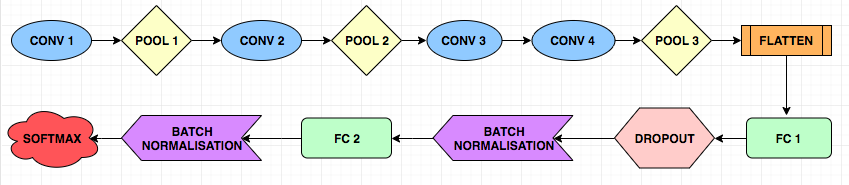
\includegraphics[scale=0.6]{flow_chart.png}
\end{center}

Relu activation function was used in all layers except for the final layer (softmax). The keep probability of dropout was set to 0.4.

\subsection{Training details}
The hyperparameters used during training are tabulated below. The code was trained first on our system and later on Google Colab.
\begin{table}[H]
	\label{T:equipos}
	\begin{center}
		\begin{tabular}{| c | c |}
			\hline
			\multicolumn{2}{|c|}{\textbf{Hyperparameters}} \\
            \hline
            Learning Rate & 0.001 \\
            Optimiser & Adam \\
            \hline
            Batch Size & 250 \\
            \hline
            Initialiser & Xavier\\
            \hline
            Activation & Relu \\
            \hline
            Epochs & 16 \\
            Patience & 5 \\
            \hline
		\end{tabular}
	\end{center}
\end{table}

%%%%%%%%%%%%%%%%%%%%%%%%%%%%% NAMIDA %%%%%%%%%%%%%%%%%%%%%%%%%%
\subsection{PLOTS}
% A plot of the learning curve showing iterations on the x-axis and negative log likelihood over labels on the y-axis. Make a single plot showing both the training loss and the validation loss.\\\\

\subsubsection{Learning Curves}
\begin{center}
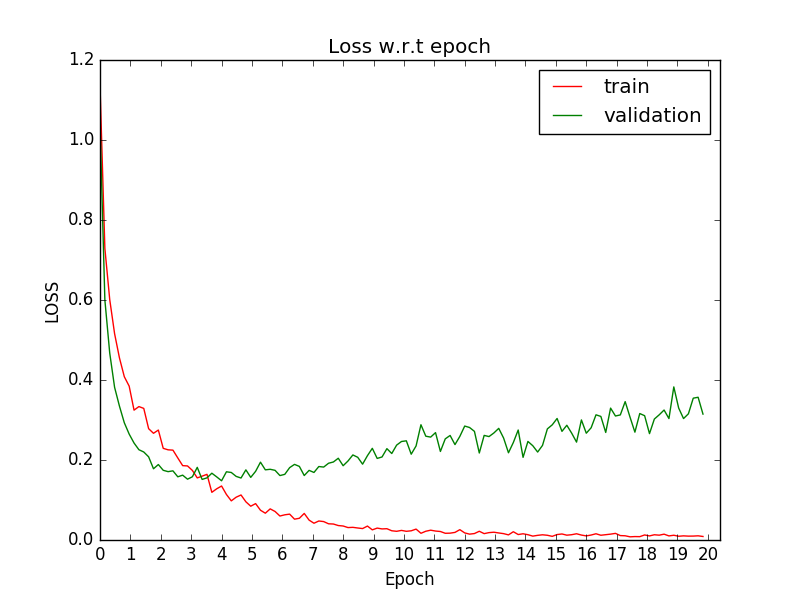
\includegraphics[scale=0.6]{loss.png}
\end{center}
\subsubsection{CONV1 filter weights}
The learned weights of the 64 filters in the first convolution layer has been plotted below. The negative weights have been given in blue and the positive weights have been given as red. The intensity of the color is a measure of the magnitude of the weights.
\begin{center}
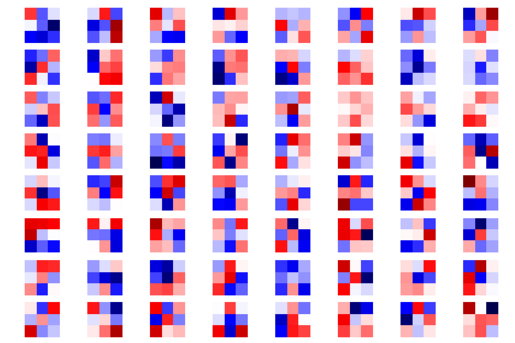
\includegraphics[scale=0.6]{filter.png}
\end{center}

\subsection{Output of Convolution layers}
The output of the filters of the convolution layers after feeding in a test image have been shown below. This allows us to study what each filter learns and analyze the trends starting from the input image to the last convolution layer.

% observe any interesting ???????????????????
As the layer progress, we notice the features extracted by each layer are more abstract compared to those of the previous layer.
We pass the following input into the network:
\begin{center}
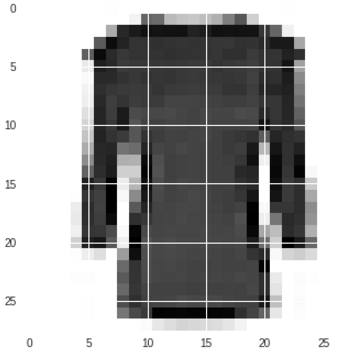
\includegraphics[scale=0.4]{input.png}
\end{center}
The activations of each layer are as follows:
\subsubsection{CONV 1}
\begin{center}
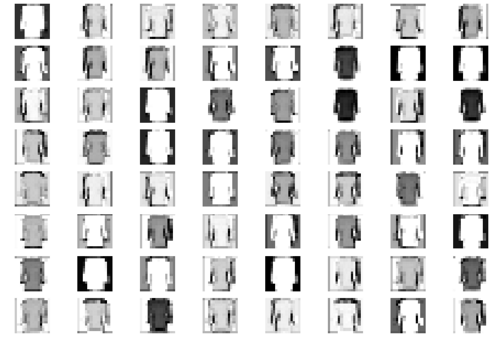
\includegraphics[scale=0.8]{conv1.png}
\end{center}

\subsubsection{CONV 2}
\begin{center}
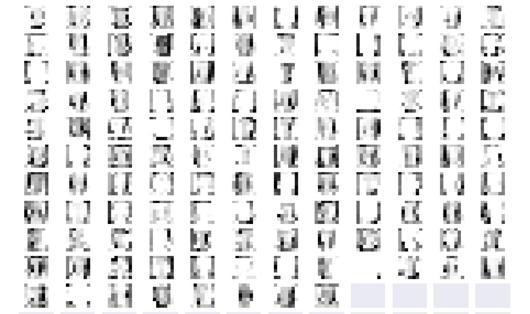
\includegraphics[scale=0.8]{con2.png}
\end{center}

\subsubsection{CONV 3}
\begin{center}
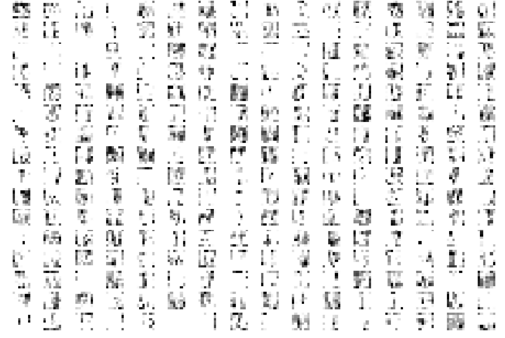
\includegraphics[scale=0.8]{conv3.png}
\end{center}

\subsubsection{CONFUSION MATRIX}
\begin{center}
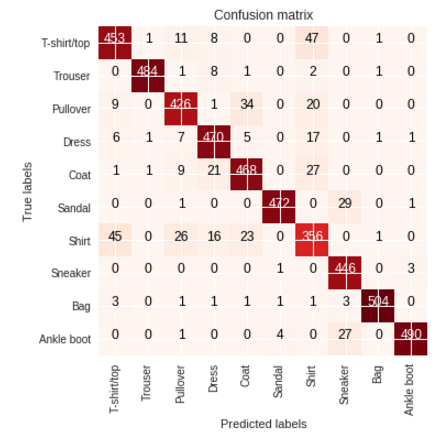
\includegraphics[scale=0.8]{confusion.png}
\end{center}

\subsection{Network specs}
%Distribution of param among fc and conv\\
As we can observe from the table given above, the one which describes the network, there are more number of parameters in the fully connected layers as compared to the convolution layers. In the considered architecture, the skewness in the distribution of parameters is relatively less. \\
The total contribution of parameters by the convolutional layers is : 959744\\
The total contribution of parameters by the dense layers is : 1117194
\begin{align*}
\textrm{Ratio } & = \frac{\textrm{No. of parameters in convolution layers}}{\textrm{No. of parameters in FC layers}}\\
				& = \frac{959744}{1117194} \\
                & = 0.859
\end{align*}


\subsection {Effect of batch norm}
To test the effect of batch normalization, the same network was considered with and without batch normalizations and was executed for 2 epochs. The dataset considered is the augmented version consisting of 1,55,000 datapoints and 1000 iterations were run for a batch size of 250. The learning rate was set as 0.001 for Adam optimiser and the activation function used was relu. The architecture followed was a slight modification of the given architecture.
\begin{table}[H]
	\label{T:equipos}
	\begin{center}
		\begin{tabular}{| c | c | c |}
			\hline
			\textbf{Batch Normalization} & \textbf{Training Accuracy} & \textbf{Validation Accuracy}\\
            \hline
            0 BN : None & 74.8 & 83.04 \\
            1 BN : Before Softmax layer & 90.4 & 89.16 \\
            2 BN : Before Softmax and output & 85.2 & 89.12 \\
            3 BN : Before Softmax, output and FC1 & 78.8 & 87.22 \\
            4 BN : Before Softmax, output, FC1, FC 2 & 84.0 & 88.92 \\
            \hline
		\end{tabular}
	\end{center}
\end{table}
It can be noticed from the table that the performance improves upon adding batch normalization to the architecture.

\subsection{Fooling the network}
 patterns\\
 plot of accuracy v/s number of pixels changed on the test set.
 
\begin{figure}[H]
\label{Images with varying levels of noise}
\centering  
\subfigure*{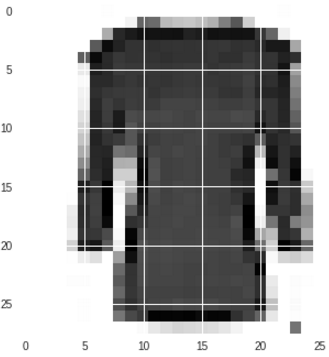
\includegraphics[width=0.235\linewidth]{1.png}}
\subfigure*{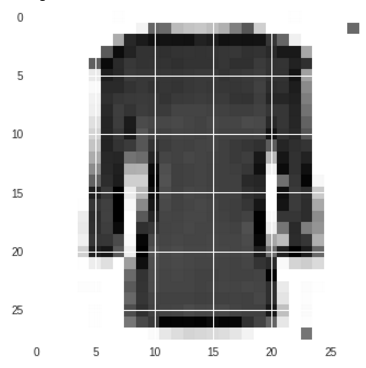
\includegraphics[width=0.25\linewidth]{2.png}}
\subfigure*{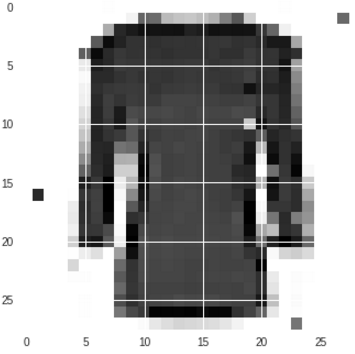
\includegraphics[width=0.25\linewidth]{3.png}}
\subfigure*{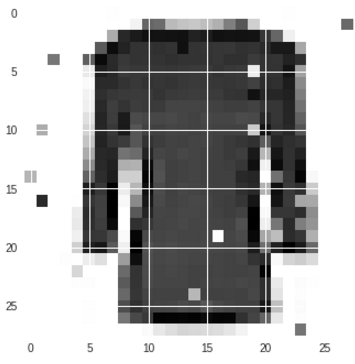
\includegraphics[width=0.25\linewidth]{4.png}}
\subfigure*{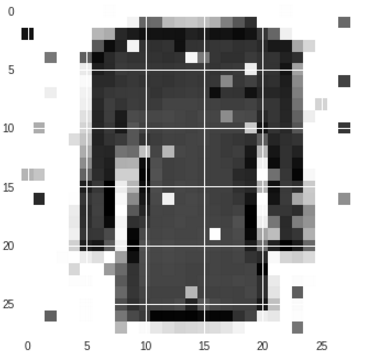
\includegraphics[width=0.25\linewidth]{5.png}}
\subfigure*{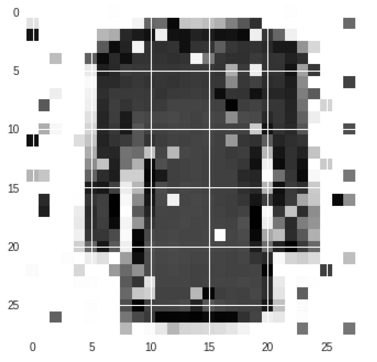
\includegraphics[width=0.25\linewidth]{6.png}}
\subfigure*{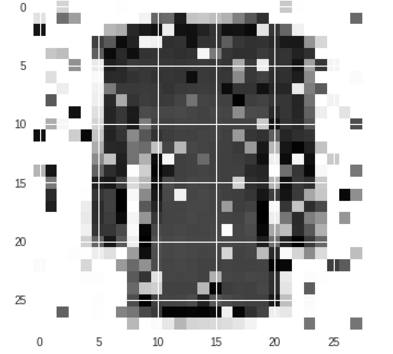
\includegraphics[width=0.25\linewidth]{7.png}}
\subfigure*{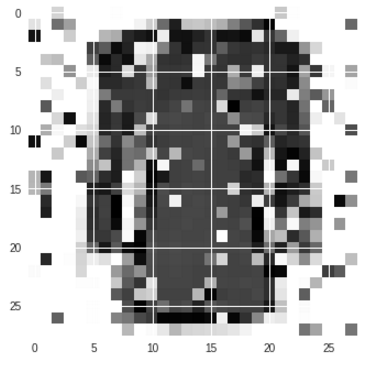
\includegraphics[width=0.25\linewidth]{8.png}}
\subfigure*{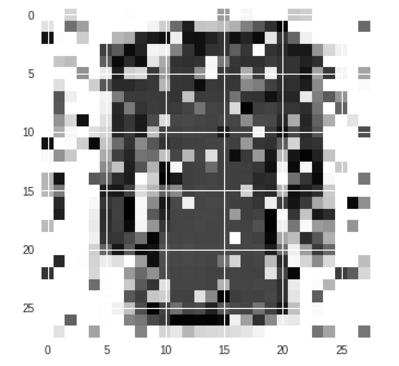
\includegraphics[width=0.25\linewidth]{9.png}}
\caption{Images with varying levels of noise}
\end{figure}[H]
 \begin{center}
 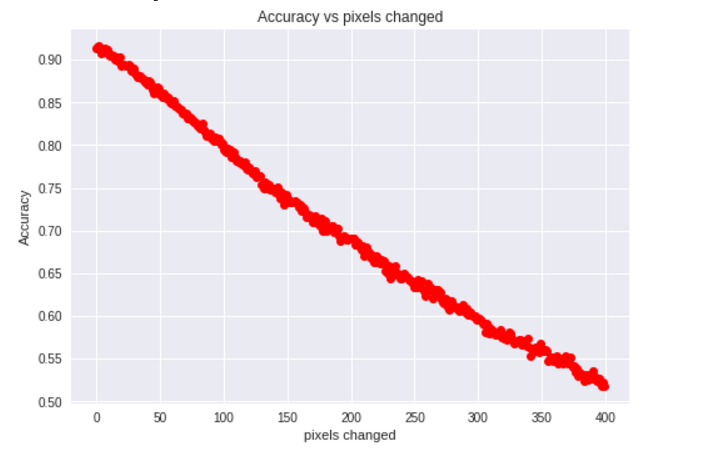
\includegraphics[scale=0.5]{fooling.png}
 \end{center}



%%%%%%%%%%%%%%%%%%%%%%%%%%%%%%%% Appendix %%%%%%%%%%%%%%%%%%%%%%%%%%
\newpage
\section{Appendix}
The following include some of the hyperparameter tuning that were carried out during the course of the assignment.

\begin{table}[H]
	\label{T:equipos}
	\begin{center}
		\begin{tabular}{| c | c |}
            \hline
            Learning Rate & $10^{-4} \ \textrm{to} \ 0.1$ \\
            \hline
            Optimisation & Adam, RMSProp A, RMSProp B \\
            \hline
            Batch Size & 500, 1000 \\
            \hline
            FC size & 256, 512, 1024 \\
            \hline
            Non Linearity & Relu, Elu \\
            \hline
            Initializer & Xavier, He \\
            \hline
		\end{tabular}
	\end{center}
\end{table}

The filtre sizes chosen varied between 7,5,3 and we found that 3 gave better accuracy and later sticked to filters of size 3 $\times$ 3.

\begin{table}[H]
	\label{T:equipos}
	\begin{center}
		\begin{tabular}{| c | c |}
            \hline
            RMSProp A & decay = 0.9 \\
            \hline
            RMSProp B & decay = 0.75, momentum = 0.01 \\
            \hline
		\end{tabular}
	\end{center}
\end{table}

\textbf{Note : } For RMSProp, selected parameters giving above 45$\%$ accuracy on validation have been shown. For Adam, values above 65$\%$ accuracy on validation have been shown. Although minor tests were run using Adagrad and Momentum based gradient descent, since Adam gave better results, further models were trained using Adam. (only Adam and RMSProp has been tabulated)\\\\
1000 iterations were run for each set of parameters with a batch size of 250.(Note : Augmented dataset)\\\\
We also noticed that there were random behaviour with certain set of hyperparameters and such behaviours were found to be less for Rmsprop in comparison to adam
 
 

\begin{table}[H]
	\label{T:equipos}
	\begin{center}
		\begin{tabular}{| c | c | c | c | c | c | c |}
			\hline
			\textbf{Learning rate} & \textbf{batch$\_$size} & \textbf{fc$\_$1size} & \textbf{non$\_$linearity} & \textbf{optimiser} & \textbf{train acc} & \textbf{val acc}\\ 
			\hline
			\hline
			0.001 & 500 & 256 & relu & Adam & 74.58 & 71.6\\
            0.01 & 500 & 256 & relu & Adam & 63.67 & 66.98\\
            \hline
            0.001 & 1000 & 256 & relu & Adam & 70.8 & 75.94\\
            0.001 & 500 & 512 & relu & Adam & 67.8 & 74.04\\
            0.01 & 500 & 512 & relu & Adam & 74.8 & 69.4\\
            0.001 & 1000 & 512 & relu & Adam & 71.8 & 77.48\\
            0.001 & 500 & 1024 & relu & Adam & 74.0 & 77.72 \\
            0.01 & 500 & 1024 & relu & Adam & 70.8 & 73.84 \\
            0.001 & 1000 & 1024 & relu & Adam & 70.1 & 74.8 \\
            0.001 & 500 & 256 & relu & Adam & 74.58 & 71.6 \\
            \hline
            0.001 & 500 & 256 & elu & Adam & 72.2 & 78.58\\
            0.001 & 1000 & 256 & elu & Adam & 71.6 & 77.64\\
            0.001 & 500 & 512 & elu & Adam & 77.2 & 79.56 \\
            0.001 & 500 & 1024 & elu & Adam & 76.4 & 79.44 \\
            0.001 & 1000 & 1024 & elu & Adam & 54.9 & 63.99 \\
            0.01 & 1000 & 512 & relu & Adam & 65.3 & 70.89 \\
            \hline
            0.0001 & 500 & 256 & relu & Adam & 66.8 & 68.99\\
            0.0001 & 500 & 512 & relu & Adam & 69.8 & 73.82\\
            0.0001 & 1000 & 512 & relu & Adam & 60.3 & 66.22 \\
            0.0001 & 500 & 1024 & relu & Adam & 69.6 & 74.92 \\
            0.0001 & 1000 & 1024 & relu & Adam & 63.4 & 67.16 \\
            0.0001 & 500 & 256 & elu & Adam & 65.6 & 74.26 \\
            0.0001 & 1000 & 256 & elu & Adam & 62.4 & 69.28 \\
            0.0001 & 500 & 512 & elu & Adam & 70.2 & 76.3 \\
            0.0001 & 1000 & 512 & elu & Adam & 66.7 & 73.44 \\
            0.0001 & 500 & 1024 & elu & Adam & 63.6 & 72.42 \\
            0.0001 & 1000 & 1024 & elu & Adam & 66.5 & 70.92 \\
           \hline
		\end{tabular}
	\end{center}
\end{table}

\begin{table}[H]
	\label{T:equipos}
	\begin{center}
		\begin{tabular}{| c | c | c | c | c | c | c |}
			\hline
			\textbf{Learning rate} & \textbf{batch$\_$size} & \textbf{fc$\_$1size} & \textbf{non$\_$linearity} & \textbf{optimiser} & \textbf{train acc} & \textbf{val acc}\\ 
			\hline
            0.001 & 500 & 256 & relu & Rmsprop$\_$A & 55.4 & 57.94\\
            0.001 & 1000 & 256 & relu & Rmsprop$\_$A & 41.8 & 46.32\\
            0.001 & 500 & 512 & relu & Rmsprop$\_$A & 58.4 & 63.73\\
            0.001 & 500 & 512 & relu & Rmsprop$\_$A & 48.2 & 52.78\\
            0.001 & 1000 & 512 & relu & Rmsprop$\_$A & 54.9 & 61.32\\
            0.001 & 500 & 1024 & relu & Rmsprop$\_$A & 68.0 & 69.52\\
            0.01 & 500 & 1024 & relu & Rmsprop$\_$A & 48.3 & 55.6\\
            0.001 & 1000 & 1024 & relu & Rmsprop$\_$A & 46.5 & 42.93\\
            0.01 & 1000 & 1024 & relu & Rmsprop$\_$A & 46.1 & 54.93\\
            0.001 & 500 & 256 & elu & Rmsprop$\_$A & 65.2 & 70.86\\
            0.01 & 500 & 256 & elu & Rmsprop$\_$A & 59.4 & 68.87\\
            0.001 & 1000 & 256 & elu & Rmsprop$\_$A & 53.8 & 59.94\\
            0.01 & 1000 & 256 & elu & Rmsprop$\_$A & 58.7 & 64.96\\
            0.001 & 500 & 512 & elu & Rmsprop$\_$A & 64.4 & 68.58\\
            0.01 & 500 & 512 & elu & Rmsprop$\_$A & 61.8 & 64.78\\
            0.001 & 1000 & 512 & elu & Rmsprop$\_$A & 58.7 & 66.52\\
            0.001 & 500 & 1024 & elu & Rmsprop$\_$A & 62.2 & 67.76\\
            0.01 & 500 & 1024 & elu & Rmsprop$\_$A & 60.8 & 67.54\\
            0.001 & 1000 & 1024 & elu & Rmsprop$\_$A & 37.5 & 57.62\\
            0.01 & 1000 & 1024 & elu & Rmsprop$\_$A & 56.7 & 63.4\\
			\hline
            0.0001 & 500 & 256 & relu & Rmsprop$\_$A & 60 & 65.26\\
            0.0001 & 500 & 1024 & relu & Rmsprop$\_$A & 63 & 68.4\\
            0.0001 & 500 & 256 & elu & Rmsprop$\_$A & 74.2 & 77.1\\
            0.0001 & 1000 & 256 & elu & Rmsprop$\_$A & 63.8 & 69.98\\
            0.0001 & 500 & 512 & elu & Rmsprop$\_$A & 63.8 & 70.2\\
            0.0001 & 500 & 1024 & elu & Rmsprop$\_$A & 64.8 & 70.94\\
            0.0001 & 1000 & 1024 & elu & Rmsprop$\_$A & 60 & 65.82\\
			\hline
		\end{tabular}
	\end{center}
\end{table}


\begin{table}[H]
	\label{T:equipos}
	\begin{center}
		\begin{tabular}{| c | c | c | c | c | c | c |}
			\hline
			\textbf{Learning rate} & \textbf{batch$\_$size} & \textbf{fc$\_$1size} & \textbf{non$\_$linearity} & \textbf{optimiser} & \textbf{train acc} & \textbf{val acc}\\ 
			\hline
            0.001 & 500 & 256 & relu & Rmsprop$\_$B & 74.6 & 77.79\\
            0.001 & 500 & 512 & relu & Rmsprop$\_$B & 48 & 56.14\\
			0.001 & 500 & 1024 & relu & Rmsprop$\_$B & 71.8 & 79.2\\
            0.001 & 500 & 256 & elu & Rmsprop$\_$B & 56.8 & 61.91\\
            0.001 & 1000 & 256 & elu & Rmsprop$\_$B & 41.9 & 47.52\\
            0.001 & 500 & 512 & elu & Rmsprop$\_$B & 47.2 & 54.88\\
            0.001 & 1000 & 512 & elu & Rmsprop$\_$B & 40.2 & 46.58\\
            0.001 & 1000 & 1024 & elu & Rmsprop$\_$B & 46.5 & 42.93\\
            0.001 & 500 & 1024 & elu & Rmsprop$\_$B & 46.4 & 48.26\\
            0.001 & 1000 & 1024 & elu & Rmsprop$\_$B & 44 & 47.36\\
            0.01 & 1000 & 1024 & elu & Rmsprop$\_$B & 47.4 & 47.92\\
			\hline
            0.0001 & 500 & 256 & relu & Rmsprop$\_$B & 67.6 & 76.8\\
            0.0001 & 1000 & 256 & relu & Rmsprop$\_$B & 66.8 & 71.74\\
            0.0001 & 500 & 512 & relu & Rmsprop$\_$B & 71.6 & 75.96\\
            0.0001 & 1000 & 512 & relu & Rmsprop$\_$B & 70.2 & 77.89\\
            0.0001 & 500 & 1024 & relu & Rmsprop$\_$B & 75.2 & 79.32\\
            0.0001 & 1000 & 1024 & relu & Rmsprop$\_$B & 71.6 & 75.84\\
            0.0001 & 500 & 256 & elu & Rmsprop$\_$B & 69.8 & 77.98\\
            0.0001 & 1000 & 256 & elu & Rmsprop$\_$B & 72.9 & 77.54\\
            0.0001 & 500 & 512 & elu & Rmsprop$\_$B & 73.2 & 77.12\\
            0.0001 & 1000 & 512 & elu & Rmsprop$\_$B & 61.1 & 71.1\\
            0.0001 & 500 & 1024 & elu & Rmsprop$\_$B & 73.6 & 77.88\\
            0.0001 & 1000 & 1024 & elu & Rmsprop$\_$B & 55.6 & 65.36\\
			\hline
		\end{tabular}
	\end{center}
\end{table}


%-------------------------------------------------------------------------------
% REFERENCES
%-------------------------------------------------------------------------------
\begin{thebibliography}{9}
\bibitem{1} 
Mitesh M Khapra. \textit{CS7015 Deep Learning: Lecture 10}, 
Indian Institute of Technology Madras, 2018
\end{thebibliography}


\end{document}

%-------------------------------------------------------------------------------
% SNIPPETS
%-------------------------------------------------------------------------------

%\begin{figure}[!ht]
%	\centering
%	\includegraphics[width=0.8\textwidth]{file_name}
%	\caption{}
%	\centering
%	\label{label:file_name}
%\end{figure}

%\begin{figure}[!ht]
%	\centering
%	\includegraphics[width=0.8\textwidth]{graph}
%	\caption{Blood pressure ranges and associated level of hypertension (American Heart Association, 2013).}
%	\centering
%	\label{label:graph}
%\end{figure}

%\begin{wrapfigure}{r}{0.30\textwidth}
%	\vspace{-40pt}
%	\begin{center}
%		\includegraphics[width=0.29\textwidth]{file_name}
%	\end{center}
%	\vspace{-20pt}
%	\caption{}
%	\label{label:file_name}
%\end{wrapfigure}

%\begin{wrapfigure}{r}{0.45\textwidth}
%	\begin{center}
%		\includegraphics[width=0.29\textwidth]{manometer}
%	\end{center}
%	\caption{Aneroid sphygmomanometer with stethoscope (Medicalexpo, 2012).}
%	\label{label:manometer}
%\end{wrapfigure}

%\begin{table}[!ht]\footnotesize
%	\centering
%	\begin{tabular}{cccccc}
%	\toprule
%	\multicolumn{2}{c} {Pearson's correlation test} & \multicolumn{4}{c} {Independent t-test} \\
%	\midrule	
%	\multicolumn{2}{c} {Gender} & \multicolumn{2}{c} {Activity level} & \multicolumn{2}{c} {Gender} \\
%	\midrule
%	Males & Females & 1st level & 6th level & Males & Females \\
%	\midrule
%	\multicolumn{2}{c} {BMI vs. SP} & \multicolumn{2}{c} {Systolic pressure} & \multicolumn{2}{c} {Systolic Pressure} \\
%	\multicolumn{2}{c} {BMI vs. DP} & \multicolumn{2}{c} {Diastolic pressure} & \multicolumn{2}{c} {Diastolic pressure} \\
%	\multicolumn{2}{c} {BMI vs. MAP} & \multicolumn{2}{c} {MAP} & \multicolumn{2}{c} {MAP} \\
%	\multicolumn{2}{c} {W:H ratio vs. SP} & \multicolumn{2}{c} {BMI} & \multicolumn{2}{c} {BMI} \\
%	\multicolumn{2}{c} {W:H ratio vs. DP} & \multicolumn{2}{c} {W:H ratio} & \multicolumn{2}{c} {W:H ratio} \\
%	\multicolumn{2}{c} {W:H ratio vs. MAP} & \multicolumn{2}{c} {\% Body fat} & \multicolumn{2}{c} {\% Body fat} \\
%	\multicolumn{2}{c} {} & \multicolumn{2}{c} {Height} & \multicolumn{2}{c} {Height} \\
%	\multicolumn{2}{c} {} & \multicolumn{2}{c} {Weight} & \multicolumn{2}{c} {Weight} \\
%	\multicolumn{2}{c} {} & \multicolumn{2}{c} {Heart rate} & \multicolumn{2}{c} {Heart rate} \\
%	\bottomrule
%	\end{tabular}
%	\caption{Parameters that were analysed and related statistical test performed for current study. BMI - body mass index; SP - systolic pressure; DP - diastolic pressure; MAP - mean arterial pressure; W:H ratio - waist to hip ratio.}
%	\label{label:tests}
%\end{table}